\documentclass{article}
\usepackage{graphicx} % Required for inserting images
\usepackage{float}

\title{Actividad 1}
\author{FiveCoders: Gabriel Freire Parola, Matias Cabello, Jonathan Suarez, \\ Santiago Seleme, Santiago Llugany }
\date{October 2025}

\begin{document}

\maketitle

\section*{Actividades:}
\begin{enumerate}
    \item  Indica qué variables son categóricas y cuáles son numéricas.
    \item Calcula el promedio de la columna Nota.
    \item Cuenta cuántos alumnos pertenecen a la carrera Sistemas.
    \item ¿Qué estudiante tiene la mayor nota?
\end{enumerate}

\subsection*{1.}
\begin{figure}[H]
    \centering
    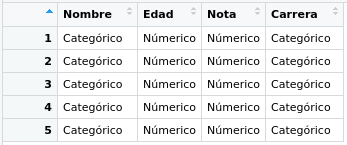
\includegraphics[width=1\linewidth]{Captura desde 2025-10-07 19-13-27.png}
    \caption{Análisis del tipo de cada elemento de la tabla}
    \label{fig:placeholder}
\end{figure}
\textbf{Podemos ver que las variables "Nombre" y "Carrera" son Categóricas, mientras que las variables "Edad" y "Nota" son Numéricas. }
\\
\subsection*{2.}
\begin{figure}[H]
    \centering
    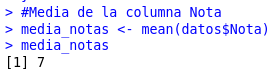
\includegraphics[width=1\linewidth]{Captura desde 2025-10-07 19-22-15.png}
    \caption{Cálculo de la media de notas}
    \label{fig:placeholder}
\end{figure}
\textbf{El promedio de las Notas es 7.}
\subsection*{3.}
\begin{figure}[H]
    \centering
    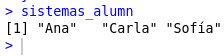
\includegraphics[width=1\linewidth]{Captura desde 2025-10-07 19-26-09.png}
    \caption{Vector filtrado alumnos que pertenecen a Sistemas}
    \label{fig:placeholder}
\end{figure}
\textbf{Ana, Carla y Sofía pertenecen a la carrera de Sistemas}

\subsection*{4.}
\begin{figure}[H]
    \centering
    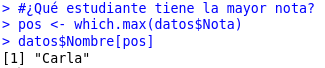
\includegraphics[width=1\linewidth]{Captura desde 2025-10-07 19-30-14.png}
    \caption{Analisis de Notas}
    \label{fig:placeholder}
\end{figure}
\textbf{Carla tiene la nota más alta}
\end{document}
